
	\section{Elastizität von Metallstäben}
	
	Der erste Versuch beschäftigt sich mit der reversiblen Elastizität von Metallstäben. Diese wird durch den Elastizitätsmodul beschrieben. Jedes Material nimmt dafür unterschiedliche Werte an, es handelt sich also um eine Materialkonstante.
	Das Ziel dieses Versuchs war, die Elastizitätsmoduln\footnote{Plural von \glqq der Elastizitätsmodul\grqq {} nach Duden} für die verwendeten Materialien zu bestimmen.
	Anschließend sollen die Ergebnisse mit den Literaturwerten verglichen werden, um das Material der Stäbe zu bestätigen.
	Da nicht gegeben ist, aus welchen Materialien die Stäbe bestehen wird vermutet, dass es sich bei diesen aufgrund der Farbe und des Gewichts um Stäbe aus Messing, Stahl und Aluminium handelt.
	
	Die Ergebnisse dieses Versuchs entsprechen den Erwartungen, also den Literaturwerten, jedoch nicht und es lässt sich keine genaue Aussage über die Materialien der Stäbe darlegen.
	
	\subsection{Methoden}	
	
	\subsubsection*{Aufbau}
	
	\begin{figure}[ht]
		\centering
		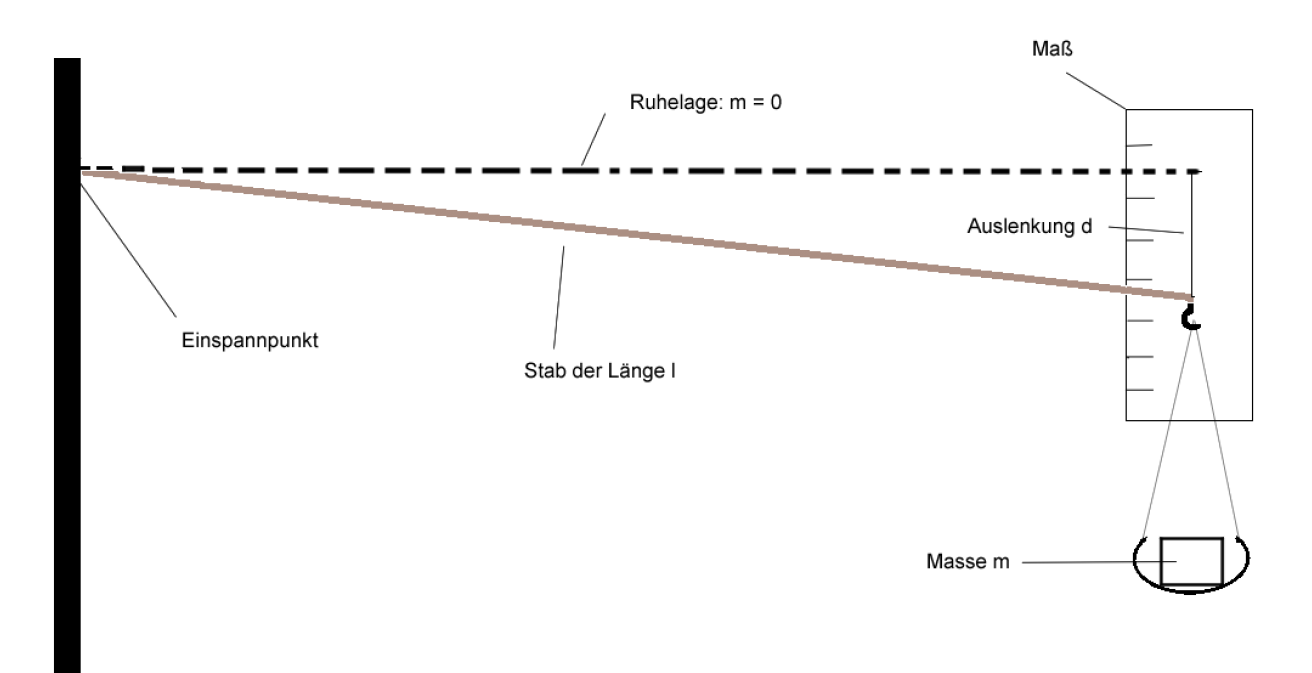
\includegraphics[width=\textwidth]{StabAuslenkungSkizze.png}
		\caption{Skizzierung des Versuchsaufbaus}
		\label{abb:Versuchsskizze1}	
	\end{figure}	
	Der Aufbau des Versuches ist in Abb. \ref{abb:Versuchsskizze1} dargestellt. Hierbei werden Stäbe aus verschiedenen Materialien eingespannt und deren Auslenkung beim Anhängen eines Gewichtes gemessen\footnote{Alle gemessenen Werte sind dem Laborbuch zu entnehmen}.
	Zudem werden Stäbe verschiedener Form untersucht.Es handelt sich bei den runden Stäben vermutlich um welche aus Messing, Stahl und Aluminium. Zusätzlich wird ein quaderförmiger Stab, vermutlich ebenfalls aus Messing, untersucht, um zu betrachten, wie sich dieser hoch- bzw. flachkant eingespannt verhält. Die Stäbe werden im Folgenden der Hypothese nach, nach ihrem Material, bezeichnet.
	Daraus wird dann der Elastizitätsmodul des jeweiligen Materials ermittelt.
	
	Mit Hilfe eines Maßbandes werden die Längen der Stäbe gemessen, die Breiten hingegen mit einer Mikrometerschraube. Um zu prüfen, ob die Stäbe an jeder Stelle die gleiche Breite besitzen, wird die Breitenmessung an fünf Stellen jeweils drei mal durchgeführt, da die Mikrometerschraube verschiedene Werte misst, je nachdem wie stark geschraubt bzw. wie fest angezogen wird. 
	Für die Messung werden pro Stab jeweils fünf verschiedene Gewichte angehängt und die Auslenkung dabei an einem Maß auf einem Spiegel parallaxenfrei abgelesen. Zur Bestimmung dieser Auslenkung, wird der Wert für die Ruhelage (bei $m=\SI{0}{\g}$) gemessen und von dem gemessenen Wert bei angehängter Masse unterschieden. Für jedes neue Gewicht wird der Wert für die Ruhelage neu bestimmt, um mögliche Ungenauigkeiten, wie durch inelastische Deformierung des Stabes, zu vermeiden.
	
	\subsubsection*{Unsicherheiten}
	
	Für die Unsicherheiten bei den Längenmessungen werden Dreiecksverteilungen verwendet. Bei der Mikrometerschraube lassen sich die Werte auf \SI{0,01}{\mm} genau ablesen, zudem war eine Unsicherheit von $10\mu $m vom Hersteller gegeben, dies wird für die Bestimmung der Unsicherheit der Mikrometerschraube verwendet. Für das Maßband und das Maß auf dem Spiegel ergibt sich dieselbe Unsicherheit, da bei beiden das Ablesen auf \SI{1}{\mm} genau möglich war.
	Die Massen waren gegeben und werden als absolut angesehen. Hier treten demnach keine Unsicherheiten auf.
	Für kombinierte Unsicherheiten wird
	\begin{equation}
	u(s) = \pm \sqrt{\sum_{k=0}^{N}\left( \frac{\partial f}{\partial x_i}u(x_i)\right) ^2} \label{eq:kombUnsicherheit}
	\end{equation}
	verwendet.
	
	\subsection{Messung}
	
	Die Messung der Länge der Stäbe ergab die in Tab. \ref{tab:Stablängen} gelisteten Werte. Hierbei wurde bei allen Stäben der Einspann von \SI{2+-0,020}{\cm} abgezogen und die Unsicherheiten kombiniert.
	\begin{table}[h]
		\caption{Länge der Stäbe}
		\centering
		\label{tab:Stablängen}
		\begin{tabular}{c|c}
			{Material} & {Länge $l$ (in cm)}\\
			\hline
			{Messing (eckig)} & {$29,2\pm 0,029$}\\
			{Messing (rund)} &  {$29,2\pm 0,029$}\\
			{Stahl} & {$28,9\pm 0,029$}\\
			{Aluminium} & {$28,6\pm 0,029$}\\		
		\end{tabular}
	\end{table}
	
	Für die Breite der Stäbe sind die gemittelten Werte für die verschiedenen Messpunkte in Tab. \ref{tab:Stabbreiten} angegeben. Auch hier ergibt sich  eine kombinierte Unsicherheit.
	\begin{table}[ht]
		\caption{Breite der Stäbe}
		\centering
		\label{tab:Stabbreiten}
		\begin{tabular}{c|c}
			\begin{tabular}{c|c}
				{Material} & {Breite (in mm)}\\
				\hline
				& {5,403}\\
				{Messing (hochkant)} & {5,397}\\
				& {5,407}\\
				& {5,410}\\
				& {5,387}\\
				\hline
				& {2,390}\\
				{Messing (flachkant)} & {2,367}\\
				& {2,363}\\
				& {2,357}\\
				& {2,403}\\
				\hline
				& {3,370}\\
				{Messing (rund)} & {3,377}\\
				& {3,400}\\
				& {3,357}\\
				& {3,403}\\
			\end{tabular}
			&
			\begin{tabular}{c|c}
				{Material} & {Breite  (in mm)}\\
				\hline
				& {3,383}\\
				{Stahl} & {3,377}\\
				& {3,380}\\
				& {3,367}\\
				& {3,387}\\
				\hline
				& {3,393}\\
				{Aluminium} & {3,390}\\
				& {3,380}\\
				& {3,373}\\
				& {3,337}\\
				\hline
				& \\ % Das soll so 
				{Unsicherheit} & \SI{+-0,011}{\mm}\\
				{für die Werte}& \\
				& \\
				& \\
			\end{tabular}		
		\end{tabular}
	\end{table}
	
	Diese Werte lassen darauf schließen, dass die Breite der Stäbe sich entlang dieser nicht merklich ändert, da alle gemessenen Werte in Bereichen innerhalb von zwei Standardunsicherheiten voneinander liegen.
	Zur Berechnung des Flächenträgheitsmoment werden die runden Stäbe deswegen als zylinderförmig angenommen.
	Dieses ergibt sich für Stäbe unterschiedlicher Querschnittsfläche wie folgt:
	\begin{align*}
	I_\text{Rechteck} = \frac{ab^3}{12} \\
	\text{bzw.} \quad I_\text{Kreis} =\frac{\pi d^4}{64}, 
	\end{align*}
	
	wobei die Seite $a$ im Falle einer rechteckigen Querschnittsfläche orthogonal zu der Biegungsebene verläuft. Die Größe $d$ entspricht dem Durchmesser bei einem kreisförmigen Querschnitt. Für $a$, $b$ und $d$ werten die oben gelisteten Breiten gemittelt. Der Durchmesser $d$ entspricht hierbei der Breite der runden Stäbe.
	
	Es ergeben sich für die Stäbe die in Tab. \ref{tab:Trägheitsmomente} aufgeführten Flächenträgheitsmomente. Hier sind die Unsicherheiten für den rechteckigen Querschnitt durch die Ableitungen von $I$ nach $a$ bzw. $b$ und deren Unsicherheiten bestimmt (vgl. Gl. \ref{eq:kombUnsicherheit}). Dasselbe gilt für die runden Stäbe, wobei hier nach $d$ abgeleitet und mit dessen Unsicherheit kombiniert wird.
	\begin{table}[ht]
		\caption{Trägheitsmomente der Stäbe}
		\centering
		\label{tab:Trägheitsmomente}
		\begin{tabular}{c|c}
			{Material} & {Trägheitsmoment $I$ (in $\text{mm}^4$)}\\ %TODO
			\hline
			{Messing (hochkant)} & {$6,037\pm 0,153$}\\
			{Messing (flachkant)} & {$31,19\pm 0,85$}\\
			{Messing (rund)} & {$6,417\pm 0,190$}\\
			{Stahl} & {$6,398\pm 0,189$} \\
			{Aluminium} & {$6,366\pm 0,189$}\\	
		\end{tabular}
	\end{table}
	Das Flächenträgheitsmoment wird benötigt um den Elastizitätsmodul zu bestimmen. Der genaue Zusammenhang ergibt sich aus der folgenden Formel für die maximale Auslenkung $h$ am Ende eines Stabes:
	\begin{equation}
	h = \frac{Fl^3}{3EI} 
	\end{equation}
	
	$F$ ist hierbei die Gewichtskraft, welche auf das Ende des Stabes wirkt. Im Folgenden wird das Eigengewicht der Stäbe bezüglich $F$ vernachlässigt.
	Da die Gewichtskraft $F = mg$ entspricht, ergibt sich ein lineares Verhältnis zwischen Auslenkung und Masse:
	\begin{equation}
	h = \frac{gl^3}{3EI}\cdot m. \label{eq:Auslenkung}
	\end{equation}
	
	Der Faktor vor $m$ entspricht also der Steigung, die man erhält, wenn man die Auslenkung der Stäbe gegen die angehängte Masse aufträgt. Die bei der dazu durchgeführten Messung erhaltenen Daten sind in Abb. \ref{abb:linearerFit} veranschaulicht.		
	Dabei weisen die gemessenen Punkte ein lineares Verhältnis auf. Da sich dieses bereits aus der Gl. \ref{eq:Auslenkung} ergab, wurden die Punkte für die verschiedenen Stäbe durch einen linearen Fit verbunden\footnote{Der Fit wurde von dem Programm SciDavis berechnet, dazu wurden die Unsicherheiten der Auslenkung und die Methode der kleinsten Quadrate herangezogen}. Die sich durch den Fit ergebenen Steigungen sind in Tab. \ref{tab:Steigungen} aufgetragen.
	\begin{figure}[ht]
		\centering
		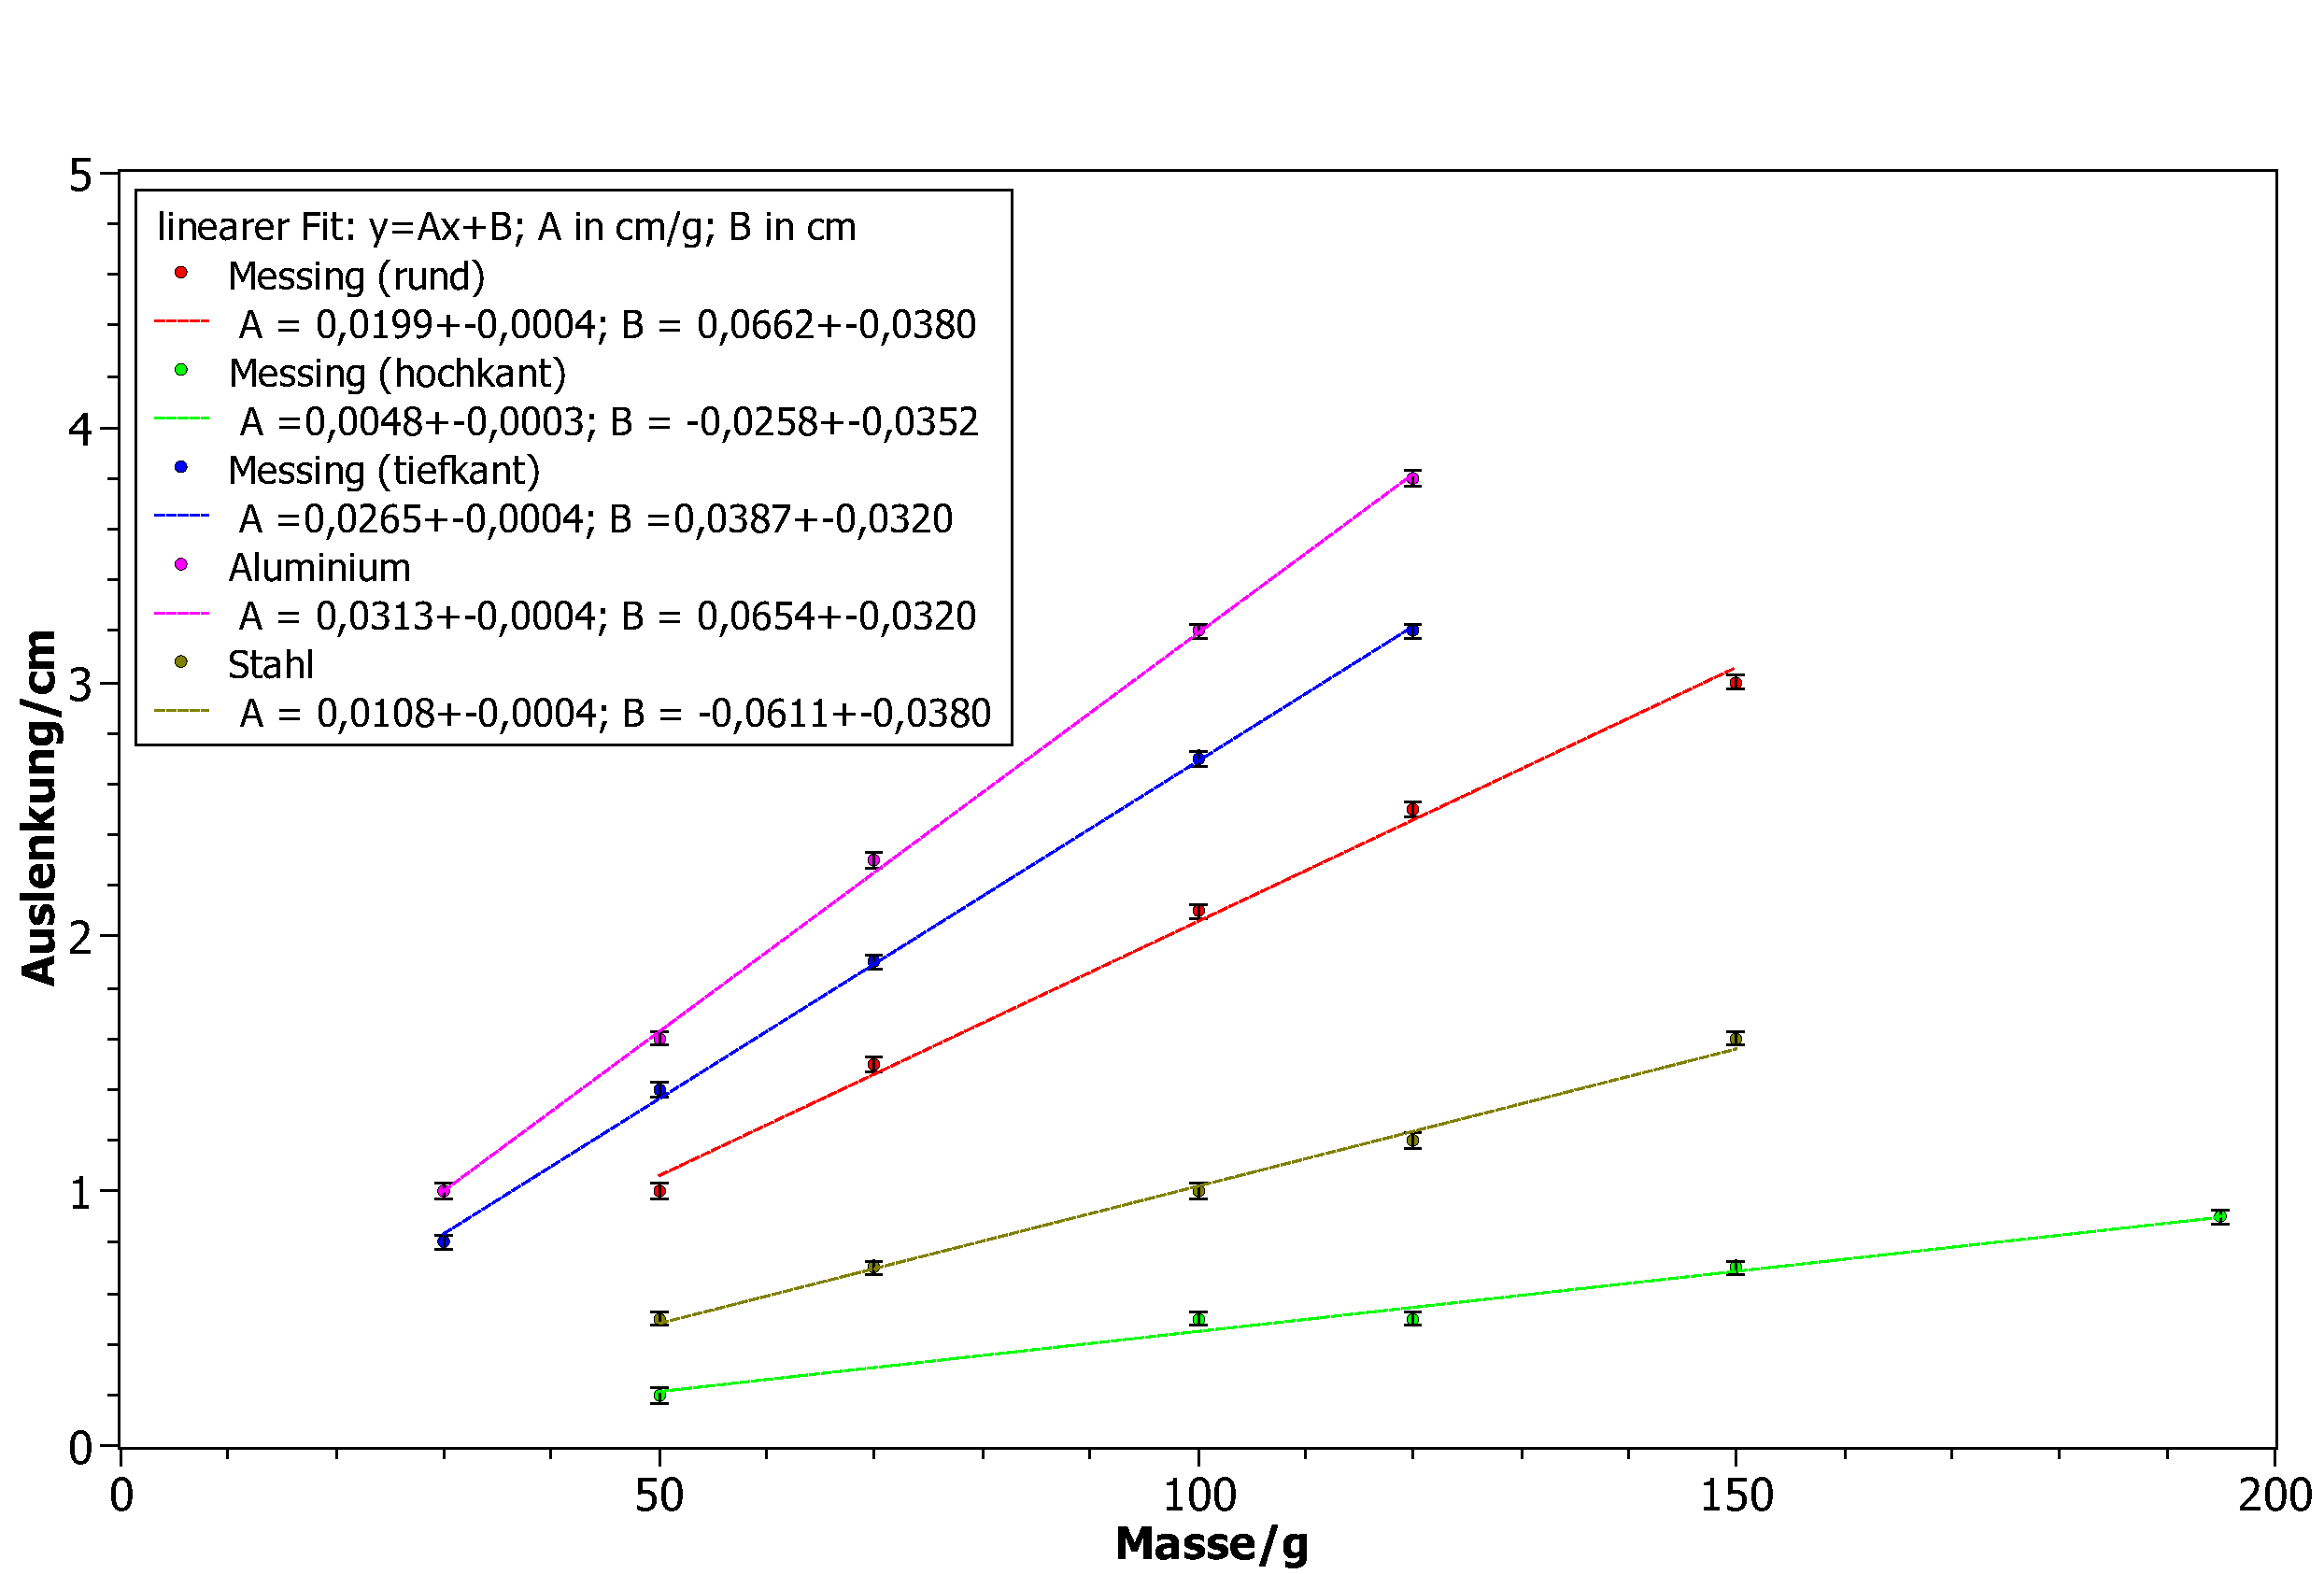
\includegraphics[width=\textwidth]{StabAuslenkungen.pdf}
		\caption{Auslenkung der Stäbe in Abhängigkeit der angehängten Masse}
		\label{abb:linearerFit}	
	\end{figure}
	\begin{table}[ht]
		\caption{Durch linearen Fit ermittelte Steigungen}
		\centering
		\label{tab:Steigungen}
		\begin{tabular}{c|c|c}
			{Material} & {Steigung $A$ (in cm/g)} & {Y-Achsenabschnitt $B$ (in cm)} \\
			\hline
			{Messing (hochkant)} & {$0,0199\pm 0,0004$} & {$0,0662\pm 0,0380$} \\
			{Messing (flachkant)} & {$0,0048\pm 0,0003$} & {$-0,0258\pm 0,0352$} \\
			{Messing (rund)} & {$0,0265\pm 0,0004$} & {$0,0387\pm 0,0320$} \\
			{Stahl} & {$0,0313\pm 0,0004$} & {$0,0654\pm 0,0320$} \\
			{Aluminium} & {$0,0108\pm 0,0004$} & {$-0,0611\pm 0,0380$} \\	
		\end{tabular}
	\end{table}
	
	Um nun den Elastizitätsmodul $E$ zu berechnen, wird der Vorfaktor von $m$ aus Gl. \ref{eq:Auslenkung}, welcher der Steigung $A$ entspricht, nach $E$ umgeformt:
	\begin{equation}
	E = \frac{gl^3}{3AI}.
	\end{equation}
	
	Einsetzen der Länge $l$, der Steigung $A$ und des Trägheitsmomentes $I$ ergeben sich für die verschiedenen Stäbe, unter Berücksichtigung der sich dabei kombinierenden Unsicherheiten, die Elastizitätsmoduln der verschiedenen Materialien. Diese sind in Tab. \ref{tab:Elastizitätsmoduln} neben den Literaturwerten aufgeführt.
	\begin{table}[ht]
		\caption{Ermittelte Elastizitätsmoduln und Literaturwerte}
		\centering
		\label{tab:Elastizitätsmoduln}
		\begin{tabular}{c|c|c}
			{Material} & {Elastizitätsmodul $E$ (in Pa)} & {Literaturwerte (in Pa)} \\
			\hline
			{Messing (hochkant)} & {($6,777\pm 0,173)\cdot 10^{10}$} & {$7,8\cdot 10^{10} \text{ bis } 12,3\cdot 10^{10}$} \\
			{Messing (flachkant)} & {($5,438\pm 0,016)\cdot 10^{10}$} & {$7,8\cdot 10^{10} \text{ bis } 12,3\cdot 10^{10}$} \\
			{Messing (rund)} & {($4,734\pm 0,142)\cdot 10^{10}$} & {$7,8\cdot 10^{10} \text{ bis } 12,3\cdot 10^{10}$} \\
			{Stahl} & {($3,941\pm 0,117)\cdot 10^{10}$} & {$9,0\cdot 10^{10} \text{ bis } 14,5\cdot 10^{10}$} \\
			{Aluminium} & {($1,113\pm 0,332)\cdot 10^{11}$} & {$7,0\cdot 10^{10}$} \\	
		\end{tabular}
	\end{table}
	
	\subsection{Diskussion}
	
	Vergleicht man die ermittelten Elastizitätsmoduln mit den Literaturwerten, so fällt auf, dass diese weit voneinander entfernt liegen.
	Zu erwarten wäre, dass der Elastizitätsmodul für das gleiche Material denselben Wert annimmt. Die Messergebnisse für die Messingstäbe liegen jedoch nicht nur weit von dem Literaturwert~\cite{1} für Messing, sondern auch voneinander. Dass die Werte, trotz geringer Unsicherheit streuen könnte bedeuten, dass es sich bei dem runden und dem eckigen Stab um verschiedene Materialien handelt, was aufgrund der Ähnlichkeit dieser bezüglich Farbe und Gewicht jedoch eher auszuschließen ist. Zumindest liegen die Werte in derselben Größenordnung und der \glqq beste\grqq {} Wert, von dem hochkant eingespannten Messingstab, liegt nur 13,2\% von dem Literaturwert entfernt. Demnach ist nicht auszuschließen, dass es sich hierbei tatsächlich um einen Messingstab handelt.
	Besonders irritierend an den Messergebnissen ist, dass der Elastizitätsmodul, welcher der Literatur nach am größten sein sollte, hier am geringsten ist und umgekehrt. Bezogen auf die Stäbe, welche vermutlich aus Stahl~\cite{2} und Aluminium~\cite{3} bestehen. Beide Elastizitätsmoduln weichen über 50\% von den Literaturwerten ab. Für den Literaturwert zum Stahl, wurde der Elastizitätsmodul von Gusseisen verwendet. Dass es sich bei dem betrachteten Stab auch um Gusseisen handelt, ist jedoch fraglich. Es ist nicht unwahrscheinlich, dass hierbei auch weitere Stoffe unter gemischt sind, deren Elastizitätsmodul von dem von Gusseisen abweicht.
	Für den Stab aus Aluminium lässt es sich jedoch nicht so argumentieren, da sein besonders leichtes Gewicht und silbrige Farbe, sowie die starke Auslenkung beim Anhängen der Gewichte deutlich auf Aluminium als Stoff weisen.
	Die Unsicherheiten sind bei allen ermittelten Elastizitätsmoduln zu klein, als dass man mit diesen näher an die Literaturwerte käme, was bei solch großen Abweichungen hilfreich wäre.
	
	\subsection{Schlussfolgerung}
	
	Aus der Ergebnisdiskussion lässt sich schließen, dass es sinnvoll wäre den Versuch zu wiederholen, da die Ergebnisse den Literaturwerten nicht entsprechen und sich demnach auch nicht erschließen ließ, ob die Stäbe aus den vermuteten Materialien bestehen. Kleinere Ungenauigkeiten könnten durch mehr Messungen vernachlässigbar werden, seien es zum Beispiel mehr Messpunkte für die Auslenkung der Stäbe oder weitere Messungen zur Breite der Stäbe mit der Mikrometerschraube. Die Ziele dieses Versuchs wurden nicht erreicht und inwieweit die Ergebnisse stimmen ist äußerst fraglich. 